\documentclass{standalone}
\usepackage{tikz}
\usetikzlibrary{calc}
\begin{document}
  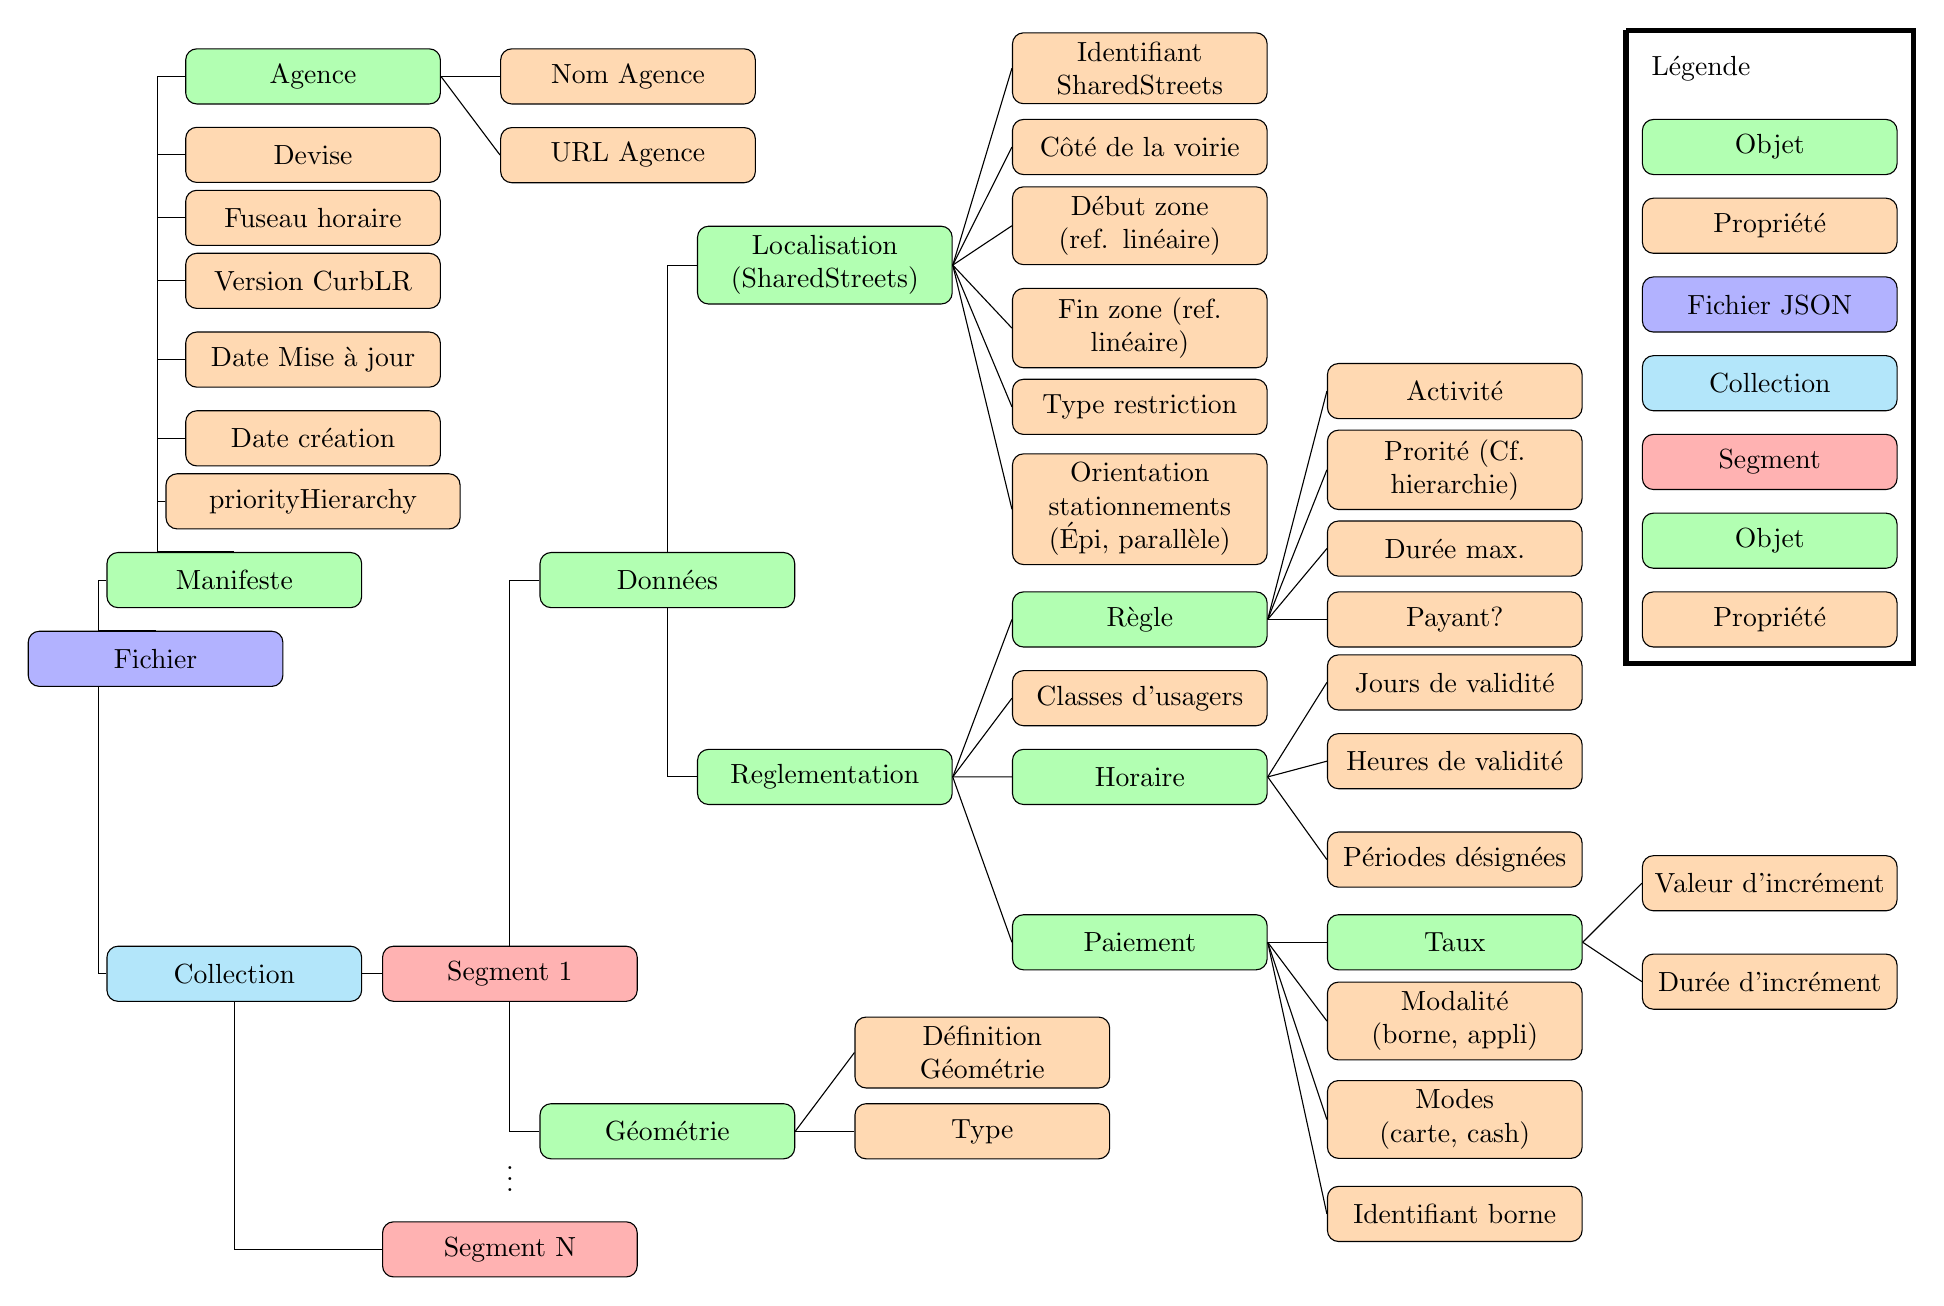
\begin{tikzpicture}
                \tikzstyle {fichier} = [rectangle, rounded corners, text width=3cm, minimum height=0.7cm,text centered,  draw=black, fill=blue!30]
                \tikzstyle {objet} = [rectangle, rounded corners, text width=3cm, minimum height=0.7cm,text centered,  draw=black, fill=green!30]
                \tikzstyle {collection} = [rectangle, rounded corners, text width=3cm, minimum height=0.7cm,text centered,  draw=black, fill=cyan!30]
                \tikzstyle {segment} = [rectangle, rounded corners, text width=3cm, minimum height=0.7cm,text centered,  draw=black, fill=red!30]
                \tikzstyle {propriete} = [rectangle, rounded corners, text width=3cm, minimum height=0.7cm,text centered,  draw=black, fill=orange!30]
                \node (fichier) [fichier] {Fichier};
                    \node (manifest) [objet,above of=fichier,xshift=1cm]{Manifeste};
                        \node (priorite) [propriete, above of=manifest,xshift=1cm,text width=3.5cm] {priorityHierarchy};
                        \draw (priorite.west) -| ++(-0.1,-0.1) |- (manifest.north);
                        \node (date_creation)[propriete, above of=priorite,yshift=-0.2cm]{Date création};
                        \draw (priorite.west) -| ++(-0.1,0.1) |- (date_creation.west);
                        \node (date_maj)[propriete,above of=date_creation]{Date Mise à jour};
                        \draw (priorite.west)  -| ++(-0.1,0.1) |- (date_maj.west);
                        \node (version) [propriete, above of=date_maj]{Version CurbLR};
                        \draw (priorite.west) -| ++(-0.1,0.1) |- (version.west);
                        \node (fuseau) [propriete,above of=version,yshift=-0.2cm]{Fuseau horaire};
                        \draw (priorite.west) -| ++(-0.1,0.1) |- (fuseau.west);
                        \node (devise) [propriete,above of=fuseau,yshift=-0.2cm]{Devise};
                        \draw (priorite.west) -| ++(-0.1,0.1) |- (devise.west);
                        \node (agence) [objet,above of=devise,yshift=-0.1]{Agence};
                        \draw (priorite.west) -| ++(-0.1,0.1) |- (agence.west);
                        \node (nom_agence) [propriete,right of=agence,xshift=3cm]{Nom Agence};
                        \draw (agence.east) -- (nom_agence.west);
                        \node (url_agence) [propriete,below of=nom_agence]{URL Agence};
                        \draw (agence.east) -- (url_agence.west);
                    \draw (manifest.west) -| ++(-0.1,-0.1) |- (fichier.north);
                    \node (coll_feature) [collection,below of=fichier,xshift=1cm,yshift=-3cm]{Collection};
                    \draw (coll_feature.west) -| ++(-0.1,0.1) |- (fichier.south);
                        \node (feature_1) [segment, right of=coll_feature,xshift=2.5cm]{Segment 1};
                        \node (feature_2) [segment, below of=feature_1,yshift=-2.5cm]{Segment N};
                        \node (ellipses) [above of=feature_2]{\vdots};
                        \draw (feature_2.west) -| (coll_feature.south);
                        \draw (coll_feature.east) -- (feature_1.west);
                            \node  (donnees) [objet,right of=feature_1,xshift=1cm,yshift=5cm]{Données};
                            \draw (donnees.west) -| (feature_1.north);
                                \node (localisation)[objet, right of=donnees,xshift=1cm,yshift=4cm]{Localisation (SharedStreets)};
                                \draw (localisation.west) -| (donnees.north);
                                    \node (id-ssr) [propriete,right of=localisation,yshift=+2.5cm,xshift=3cm]{Identifiant SharedStreets};
                                    \draw (id-ssr.west) -- (localisation.east);
                                    \node (ssr-side)[propriete,below of=id-ssr,yshift=-0cm]{Côté de la voirie};
                                    \draw (ssr-side.west) -- (localisation.east);
                                    \node (ref-lin-debut)[propriete, below of=ssr-side,yshift=-0cm]{Début zone (ref. linéaire)};
                                    \draw (ref-lin-debut.west) -- (localisation.east);
                                    \node (ref-lin-fin)[propriete,below of=ref-lin-debut,yshift=-0.3cm]{Fin zone (ref. linéaire)};
                                    \draw (ref-lin-fin.west) -- (localisation.east);
                                    \node (asset-type) [propriete, below of=ref-lin-fin,yshift=-0cm]{Type restriction};
                                    \draw (asset-type.west) -- (localisation.east);
                                    \node (bays-angle)[propriete, below of=asset-type,yshift=-0.3cm]{Orientation stationnements (Épi, parallèle)};
                                    \draw (bays-angle.west) -- (localisation.east);
                                \node (reglementation)[objet,below of=localisation,yshift=-5.5cm]{Reglementation};
                                \draw (reglementation.west) -| (donnees.south);
                                    \node (regle)[objet,right of=reglementation,xshift=3cm,yshift=+2cm]{Règle};
                                    \draw (regle.west) -- (reglementation.east);
                                        \node (payant) [propriete,right of=regle,xshift=3cm]{Payant?};
                                        \draw (payant.west) -- (regle.east);
                                        \node (duree_max)[propriete,above of=payant,yshift=-0.1cm]{Durée max.};
                                        \draw (duree_max.west) -- (regle.east);
                                        \node (priorite)[propriete, above of=duree_max,yshift=0cm]{Prorité (Cf. hierarchie)};
                                        \draw (priorite.west) -- (regle.east);
                                        \node (activite)[propriete,above of=priorite,yshift=0cm]{Activité};
                                        \draw (activite.west) -- (regle.east);
                                    \node (classes_usagers)[propriete,below of=regle,yshift=-0cm]{Classes d'usagers};
                                    \draw (classes_usagers.west) -- (reglementation.east);
                                    \node (horaire) [objet,below of=classes_usagers,yshift=0cm]{Horaire};
                                    \draw (horaire.west) -- (reglementation.east);
                                        \node (jours) [propriete,right of=horaire,xshift=3cm,yshift=1.2cm]{Jours de validité};
                                        \draw (jours.west) -- (horaire.east);
                                        \node (heures)[propriete,below of=jours,yshift=-0cm]{Heures de validité};
                                        \draw (heures.west) -- (horaire.east);
                                        \node (periodes) [propriete,below of=heures,yshift=-0.25cm]{Périodes désignées};
                                        \draw (periodes.west) -- (horaire.east);
                                    \node (paiement) [objet, below of=horaire,yshift=-1.1cm]{Paiement};
                                    \draw (paiement.west) -- (reglementation.east);
                                        \node (taux) [objet, right of=paiement,xshift=3cm]{Taux};
                                        \draw (taux.west) -- (paiement.east);
                                            \node (val_increment)[propriete,right of=taux,xshift=3cm,yshift=0.75cm]{Valeur d'incrément};
                                            \draw (val_increment.west) -- (taux.east);
                                            \node (dur_increment) [propriete,below of=val_increment,yshift=-0.25cm]{Durée d'incrément};
                                            \draw (dur_increment.west) -- (taux.east);
                                        \node (modalite)[propriete,below of=taux,yshift=-0cm]{Modalité (borne, appli)};
                                        \draw (modalite.west) -- (paiement.east);
                                        \node (methode) [propriete,below of=modalite,yshift=-0.25cm]{Modes (carte, cash)};
                                        \draw (methode.west) -- (paiement.east);
                                        \node (id_modul)[propriete,below of=methode,yshift=-0.2cm]{Identifiant borne};
                                        \draw (id_modul.west)-- (paiement.east);
                            \node (geometrie) [objet,below of=donnees,yshift=-6cm]{Géométrie};
                            \draw (geometrie.west) -| (feature_1.south);
                                \node (type_geo) [propriete, right of=geometrie,xshift=3cm]{Type};
                                \draw (type_geo.west) -- (geometrie.east);
                                \node (def_geo) [propriete,above of=type_geo,]{Définition Géométrie};
                                \draw (def_geo.west) -- (geometrie.east);
                \node (legend) [right of=id-ssr, text width=3cm,xshift=7cm]{Légende};
                \coordinate (boite_top_left)at($(legend.north west)+ (-0.2,0.2)$);
                \node (objet_desc)[objet,below of=legend]{Objet};
                \node (propriete_desc) [propriete,below of=objet_desc]{Propriété};
                \node (fichier_desc) [fichier, below of=propriete_desc]{Fichier JSON};
                \node (collection_desc) [collection, below of=fichier_desc]{Collection};
                \node (caracteristique_desc) [segment, below of=collection_desc]{Segment};
                \node (objet_desc) [objet,below of=caracteristique_desc]{Objet};
                \node (propriete_desc) [propriete, below of=objet_desc]{Propriété};
                \coordinate (boite_bot_rght) at ($(propriete_desc.south east)+ (0.2,-0.2)$);
                \draw[line width=2pt] (boite_top_left) -| (boite_bot_rght) -| (boite_top_left);    
             \end{tikzpicture}

\end{document}